\subsection{Oriented FAST and Rotated BRIEF (ORB)}
Das folgende Kapitel basiert auf dem von Ethan Ruble veröffentlichtem Paper ''ORB: an efficient alternative to SIFT or SURF'' \footnote{\cite{Rublee:2011:OEA:2355573.2356268,}}.

ORB wurde 2011 von Ethan Ruble als eine alternative zu SIFT und SURF vorgestellt, die deutlich schneller sein und dabei jedoch eine vergleichbar gute Perfomance haben sollte.
ORB kombiniert mehrere bestehende Verfahren und erweitert diese, um mit Rotation umgehen zu können. So wird FAST und ein Harris-Corner Detector \footnote{\cite{Harris88alvey}} verwendet, um Keypoints zu finden. Zudem werden die ''Binary Robust Independent
Elementary Features'' (BRIEF) \footnote{\cite{Calonder:2010:BBR:1888089.1888148,}} für die Merkmalsbeschreibung verwendent und so erweitert, dass sie mit der Rotation von Bildausschnitten umgehen können.

\subsubsection{Merkmalserkennung}

Um eine erste Auswahl an möglichen Keypoints zu erhalten wird FAST (siehe \ref{sec:fast}) verwendet.


FAST findet jedoch auch viele Punkte, die an einer Kante liegen und keine Ecke sind. Um diese herauszufiltern, wird der Harris-Corner Detector verwendet. Dieser gibt für einen Punkt ein Maß an, wie sehr dieser Punkt eine Ecke ist \footnote{\cite{Harris88alvey}}.


Für alle von FAST gefundenen Punkte wird der Harris Wert berechnet.
Um eine gewisse Anzahl $N$ an Punkten zu finden, wird  eine Schwelle $t$ zuerst so klein gewählt, dass mehr als $N$ Punkte über dieser liegen. Diese Punkte werden dann nach ihrem Harris Wert geordnet und die $N$ größten ausgewählt.
Damit die Merkmale Skalierungsinvariant sind, wird dies für mehrer Skalierungen des Bildes durchgeführt.

Da die von FAST gefundenen Punkte keine Orientierung haben, wird jedem gefundenen Merkmal noch eine Orientierung zugewiesen.
Dafür wird der Intensitätsschwerpunkt genutzt. Dieser liegt bei einer Ecke versetzt vom Mittelpunkt des betrachteten Bildausschnitts.
Um den Intensitätsschwerpunkt zu finden, werden die Momente des Ausschnittes betrachtet.
Momente in der Bildverarbeitung sind gewichtetete Intensitäten der Pixel eines Bildes bzw. eines Bildausschnittes.
Der Moment des $p$ und $q$ Grades, mit $p, q \in \mathbb{R}$ ist definiert als:

\[
m_{pq} = \sum_{x, y} x^p y^q I(x, y)
\]

Aus den Momenten $m_{00}, m_{01}$ und $m_{10}$ lässt sich der Schwerpunkt bestimmen.

\[
C =  \bigg(\frac{m_{10}}{m_{00}} , \frac{m_{01}}{m_{00}}\bigg)
\]

Die Orientierung des Keypoints wird definiert als der Vektor vom Zentrum bis zum Intensitätsschwerpunkt (siehe Abbildung \ref{fig:centroid}).

\begin{figure}[h]

    \centering
		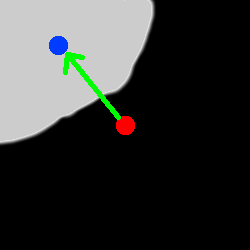
\includegraphics[scale=0.65]{bilder/centroid.png}
    	\caption{Der rote Punkt ist das Zentrum des Bildausschnitts und der blaue Punkt markiert den Intensitätsschwerpunkt. Der grüne Vektor zwischen den beiden bestimmt die Orientierung des Bildausschnitts.}
\label{fig:centroid}
\end{figure}


\[
\theta = \atantwo (m_{01}, m_{10})
\]

Diese Orientierung wird in $2\pi / 30$ große Abschnitte unterteilt.

\subsubsection{Merkmalsbeschreibung}

Um einen Deskriptor für ein gefundenes Merkmal zu bilden, wird ein $31 \times 31$ Bildausschnitt $p$ um den Keypoint betrachtet.
ORB benutzt eine um Rotation erweiterte Variante von BRIEF.
BRIEF erstellt einen binären Vektor aus einfachen Intensitätsvergleichen von zwei Bildpunkten. Hierfür wird der Bildausschnitt $p$ zuerst mit einem Gaußfilter geglättet.

Der binäre Test $\tau$ für den Bildausschnit $p$, wobei $p(x)$ die Intenstität an Bildpunkt x ist, ist definiert als:

\[
\tau(p; x, y) = 
\begin{cases}
1, & p(x) < p(y) \\
0, & p(x) \geq p(y)
\end{cases}
\]

Die Bitfolge der Testergebnisse ergibt sich aus:

\[
f_n(p) = \sum_{1 \leq i \leq n} 2^{i-1} \tau (p; x_i, y_i)
\]



Definiere die $2 \times n$ Matrix $S$ für alle n Vergleichspunkte $(x_i, y_i)$:

\[
S = \begin{pmatrix}
x_1 & \hdots & x_n \\
y_1 & \hdots & y_n 
\end{pmatrix}
\]

Für den Winkel $\theta$ des Bildausschnitts wird die Rotationsmatrix $R_\theta$ definiert, welche die Punkte in $S$ um $\theta$ dreht.

\[
S_\theta = R_\theta S
\]


\[
g_n(p, \theta) = f_n(p)|(x_i, y_i) \in S_\theta
\]


In der $31 \times 31$ Umgebung um den Keypoint gibt es eine hohe Anzahl an Bildpunkten, die miteinander verglichen werden könnten. Von all diesen Paaren $(x, y)$ sollen 256 ausgewählt werden.
Damit der Deskriptor möglichst diskriminierend ist, sollen Paare gewählt werden, die für eine große Menge an Bildausschnitten, auf denen sie ausgeführt werden, folgenden Eigenschaften haben:
\begin{itemize}

\item  Der Mittelwert des Testergebnisses liegt möglichst nah an $0.5$, also liefert der Test für verschiedene Bilder oft verschiedene Ergebnisse

\item Die Korrelation zwischen den gewählten Tests sollte möglichst gering sein, sodass jeder Test neue Informationen hinzubringt

\end{itemize}

Um die Testpaare zu lernen nutzt ORB ein Trainingsset von ca. 300000 Merkmalen aus dem PASCAL 2006 Bildersatz. Eine Auswahl der gelernet Testpaare ist in Abbildung \ref{fig:orbPairs} dargestellt.

\begin{figure}[h]

    \centering
		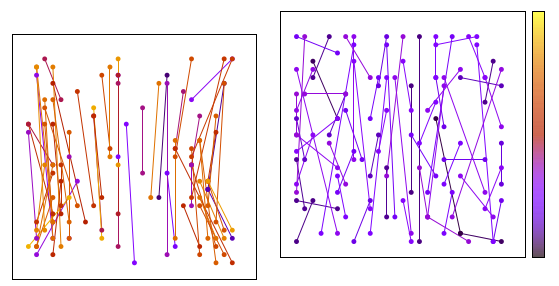
\includegraphics[scale=0.5]{bilder/orbPairs.png}
    	\caption{Darstellung einer Auswahl an Testpaaren. Die linke Seite zeigt Testpaare, die eine hohe Varianz besitzen. Die rechte Seite zeigt die Tests, nachdem der Trainingsschritt abgeschlossen wurde. Die Farben zeigen die maximale Korrelation eines Tests an. Schwarz und Lila stellen die geringste Korrelation dar. }
\label{fig:orbPairs}
\end{figure}

Es werden zuerst alle möglichen Testpaare für alle Keypoints berechnet und nach dem Abstand ihres Mittelwertes zu $0.5$ sortiert. 
Zunächst wird der Test, dessen Mittelwert am nächsten an $0.5$ dran ist, in die Ergebnismenge hinzugefügt.


Nun wird die sortierte Liste an Testpaaren durchgelaufen und ein Test zur Ergebnissmenge hinzugefügt wenn, seine Korrelation unter einem Schwellwert liegt. Ist das der Fall, wird der Test aus der sortierten Liste entfernt. Dies wird solange durchgeführt bis 256 Tests in der Ergebnismenge sind. 
Wird die Liste komplett durchlaufen und die Ergebnismenge ist kleiner als 256, wird der Schwellwert verringert und die Liste noch einmal neu durchlaufen.

Die so gefundenen 256 Testpaare bilden nun den ORB Deskriptor.